\chapter{Организационно-экономическая часть}
Организация и планирование процесса разработки программного обеспечения предусматривает выполнение следующих задач:
\begin{enumerate}[1.]
\item формирование состава выполняемых работ и группировка их по стадиям разработки;
\item расчет трудоемкости выполнения работ;
\item расчет количества исполнителей;
\item построение сетевого графика;
\item разработка календарного графика работ;
\item Анализ структуры затрат проекта;
\item Оценка экономической целесообразности проекта;
\end{enumerate}

\section{Основные этапы разработки программного продукта}
Разработку программного продукта разбивают на следующие стадии:
\begin{enumerate}[1.]
\item \textbf{Техническое задание.} Постановка задач. Определение пакета прикладных программ, состава и структуры информационной базы. Выбор языков программирования. Предварительный выбор методов выполнения работы. Разработка календарного плана выполнения работ.
\item \textbf{Эскизный проект.} Предварительная разработка структуры входных и выходных данных. Разработка общего описания алгоритмов решения задач. Разработка пояснительной записки. Согласование и утверждение эскизного проекта.
\item \textbf{Технический проект.} Разработка алгоритмов решения задач. Разработка пояснительной записки. Согласование и утверждение технического проекта. Разработка структуры программы. Разработка программной документации и передача ее для включения в технический проект. Внесение правок в структуры, анализ и определение формы представления входных и выходных данных. Выбор конфигурации технических средств.
\item \textbf{Рабочий проект.} Комплексная отладка задач и сдача в опытную эксплуатацию. Разработка проектной документации. Программирование и отладка программ. Описание контрольного примера. Разработка программной документации. 
\item \textbf{Внедрение.} Подготовка и передача программной документации для сопровождения с оформлением соответствующего акта. Передача программной продукции в фонд алгоритмов и программ. Проверка алгоритмов и программ решения задач, корректировка документации после опытной эксплуатации программного продукта.
\end{enumerate}

Анализирую требования ГОСТ, можно предложить следующее распределение работ по этапам:
\begin{enumerate}[1.]
\item Разработка технических требований, предъявляемых к разрабатываемому ПО и проведение исследований заданной области.
\item Разработка алгоритмов работы ПО, выбор среды программирования.
\item Разработка программных модулей (написание кода).
\item Тестирование и отладка разрабатываемого ПО.
\item Разработка документации.
\end{enumerate}

Этап внедрения отсутствует, так как разрабатываемое ПО будет внедряться силами заказчиков данного ПО без участия разработчиков.

\section{Расчет трудоемкости проекта}
Определим вероятные трудозатраты на выполнение данного проекта. Существует несколько методик опеределния трудозатрат, воспользуемся опеределением с помощью экспертных оценок. Для этой цели было опрошено четверо экспертов-разработчиков в области сетевых технологий.

В Таблице~\ref{table:expert_marks} приведены оценки экспертов:

\begin{table}
\centering
\caption{Экспертные оценки}
\label{table:expert_marks}
\begin{tabular} {| c | c |} 
\hline
Эксперт 1 & 500\\
\hline
Эксперт 2 & 400\\
\hline
Эксперт 3 & 650\\
\hline
Эксперт 4 & 700\\
\hline
\end{tabular}
\end{table}

Общие затраты труда на разработку определим следующим образом:
\begin{equation}
Q_{P} = \sum_{i}t_i,
\end{equation}
где $t_{i}$ - затраты труда на выполнение i-го проекта.

Используя метод экспертных оценок, вычислим ожидаемую продолжительность работ T каждого этапа по формуле:
\begin{equation}
T = \frac{3 \cdot T_{MIN} + 2 \cdot T_{MAX}} {5} = \frac{3 \cdot 400 + 2 \cdot 700} {5} = 520,
\end{equation}
где $T_{MIN}$ - минимальная продолжительность работ, $T_{MAX}$ - максимальная продолжительность работ;

Продолжительности работ назначаются в соответствии с экспертными оценками, а ожидаемая продолжительность работы рассчитывается как математическое ожидание для $\beta$-распределения.

Полный перечень работ с разделением по этапам приведен в Таблице~\ref{table:all_works}.
\begin{table}
\caption{Перечень работ}
\label{table:all_works}
\begin{tabular} {| p{0.15\textwidth} | p{0.08\textwidth} | p{0.3\textwidth} | p{0.1\textwidth} | p{0.1\textwidth} | p{0.1\textwidth} | p{0.09\textwidth} |} 
\hline
Этап & № & Содержание & $T_{MIN}$, & $T_{MAX}$, & T, & T, \\
& работы & работы & чел/часы & чел/часы & чел/часы & чел/дни\\
\hline
\multirow{4}{\hsize}{Разработка технических требований}
& 1 & Согласование списка поддерживаемых протоколов & 8 & 8 & 8 & 1\\
\cline{2-7}
& 2 & Разработка и утверждение ТЗ & 16 & 36 & 24 & 3\\
\cline{2-7}
& 3 & Анализ предметной области и существующих решений & 20 & 30 & 24 & 3\\
\cline{2-7}
& 4 & Анализ фреймворка DPDK и его возможностей & 16 & 16 & 16 & 2\\
\hline
\multirow{3}{\hsize}{Описание структур данных и алгоритмов}
& 5 & Разработка файла конфигурации: синтаксис, поддерживаемые действия, допустимые значения & 48 & 68 & 56 & 7\\
\cline{2-7}
& 6 & Разработка алгоритмов обнаружения протоколов & 72 & 92 & 80 & 10\\
\hline
\multirow{2}{\hsize}{Разработка программных модулей}
& 7 & Реализация модуля работы с файлом конфигурации & 60 & 70 & 64 & 8\\
\cline{2-7}
& 8 & Реализация главного модуля обработки сетевого трафика & 90 & 145 & 112 & 14\\
\hline
\multirow{3}{\hsize}{Тестирование и отладка ПО}
& 9 & Тестирование функциональности & 32 & 52 & 40 & 5\\
\cline{2-7}
& 10 & Тестирование производительности & 24 & 24 & 24 & 3 \\
\hline
Разработка документации & 12 & Написание программной и эксплуатационной документации & 66 & 81 & 72 & 9\\
\hline
\end{tabular}
\end{table}

Итого: $Q_{\textup{Р}} = Q_{\textup{ОЖ}} = 65 \textup{чел/дней} = 520 \textup{чел/час}$

\section{Определение численности исполнителей}
Средняя численность исполнителей определяется по формуле:
\begin{equation}
N = \frac{Q_{P}} {F},
\end{equation}
где F - фонд рабочего времени и определяется по формуле:
\begin{equation}
F = \sum_{i}^r F_{Mi} = \sum_{i}^r (D_{\textup{о}} - D{ \textup{в}} - D_{\textup{п}}),
\end{equation}
где $F_{Mi}$ - фонд времени в текущем i-том месяце и вычисляется для каждого месяца с учетом количества праздников $D_{\textup{о}}$, выходных $D_{\textup{в}}$ и праздничных $D_{\textup{п}}$ дней.

На реализацию проекта отведено r = 3 месяца рабочего времени при односменной работе с продолжительностью рабочего времени 8 часов. В Таблице~\ref{table:time_fond} приведены сведения, необходимые для вычисления фонда времени для каждого месяца и итоговые результаты вычислений.
\begin{table}
\caption{Месячный фонд времени}
\label{table:time_fond}
\begin{tabular} {| p{0.1\textwidth} | p{0.2\textwidth} | p{0.15\textwidth} | p{0.15\textwidth} | p{0.15\textwidth} | p{0.15\textwidth} |} 
\hline
Месяц & Количество & Количество & Количество & Фонд & Фонд\\
& дней & выходных & праздничных & времени & времени \\
& & дней & дней & $F_{Mi}$,  дни & $F_{Mi}$, дни\\
\hline
Февраль & 29 & 8 & 1 & 20 & 159\\
\hline
Март & 31 & 9 & 1 & 21 & 168\\
\hline
Апрель & 30 & 9 & 0 & 21 & 168\\
\hline
\end{tabular}
\end{table}

Таким образом, фонд рабочего времени проекта составляет  F = 495 часов.

Отсюда средняя численность исполнителей равна:
\begin{equation}
N = \frac{Q_{P}} {F} = \frac{520} {495} = 1.05
\end{equation}

Таким образом, по суммарным трудозатратам для завершения проекта в заданные сроки необходимо два исполнителя: инженер и программист. Учитывая специфику дипломного проекта, данные специалисты должны обладать знаниями в следующих областях:
\begin{itemize}
\item протоколы вычислительных сетей;
\item сетевое программирование;
\item высокопроизводительные информационные системы и комплексы;
\item разработка алгоритмов и архитектуры ПО;
\item тестирование ПО;
\item разработка документации;
\end{itemize}

\section{Построение сетевого графика}
Для определения временных затрат и трудоемкости разработки ПО используем метод сетевого планирования. Этот метод позволяет установить единой схемой связь между всеми работами в виде наглядного и удобного для восприятия изображения (сетевого графика), представляющего собой информационно-динамическую модель, позволяющую определить продолжительность и трудоемкость как отдельных этапов, так и всего комплекса работ в целом.

Составление сетевой модели включает в себя оценку степени детализации комплекса работ и определения логической связи между отдельными работами. С этой целью составляется перечень всех основных работ и событий. В перечне указываются кодовые номера событий, наименования событий в последовательности от исходного к завершающему, кодовые номера работ, перечень всех работ, причем подряд указываются все работы, которые начинаются после наступления данного события.

Основные событий и работы представлены в Таблице~\ref{table:events_and_works}.
\begin{longtable}{| p{0.03\textwidth} | p{0.33\textwidth} | p{0.1\textwidth} | p{0.3\textwidth} | p{0.07\textwidth} | p{0.07\textwidth} |} 
\caption{Основные работы и события проекта}
\label{table:events_and_works}
\\ \hline
$N_{i}$  & Наименование события & Код & Работа & t, & t,\\
& & работы & & чел/ч & чел/д \\
\hline \endfirsthead
\subcaption{Продолжение таблицы~\ref{table:events_and_works}}
\\ \hline \endhead
\hline \subcaption{Продолжение на след. стр.}
\endfoot
\hline \endlastfoot

0 & Разработка ПО начата & 0-1 & Согласование списка поддерживаемых протоколов & 8 & 1\\
\hline
1 & Протоколы согласованы & 1-2 & Разработка и утверждение ТЗ & 24 & 3\\
\hline
2 & ТЗ разработано и утверждено & 2-3 & Анализ предметной области и существующих решений & 24 & 3\\
\hline
3 & Анализ существующих решений проведен & 3-4 & Анализ фреймворка DPDK & 16 & 2\\
\hline
4 & DPDK проанализирован & 4-5 & Разработка файла конфигурации & 56 & 7\\
\cline{3-6}
& & 4-6 & Разработка алгоритмов обнаружения & 80 & 10\\
\hline
5 & Описание файла конфигурации выполнено & 5-6 & Фиктивная работа & 0 & 0\\
\hline
6 & Алгоритмы разработаны & 6-7 & Реализация модуля конфигурации & 64 & 8\\
\hline
7 & Модуль файла конфигурации реализован & 7-8 & Реализация главного модуля & 112 & 14\\
\hline
8 & Главный модуль реализован & 8-9 & Тестирование функциональности & 40 & 5\\
\cline{3-6}
& & 8-10 & Тестирование производительности & 24 & 3\\
\hline
9 & Функциональность протестирована & 9-11 & Разработка документации & 72 & 9\\
\hline
10 & Производительность протестирована & 10-12 & Фиктивная работа & 0 & 0\\
\hline
11 & Документация разработана & 11-12 & Фиктивная работа & 0 & 0\\
\hline
12 & Разработка ПО завершена & - & - & - & -\\

\end{longtable}

Сетевой график приведен на Рисунке~\ref{fig:netgraph}.
\begin{figure}
\caption{Сетевой график}
\label{fig:netgraph}
\centering
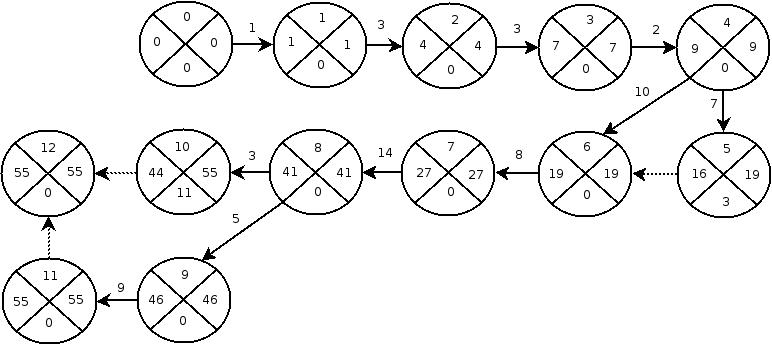
\includegraphics[scale=0.5]{pictures/netgraph}
\end{figure}

\section{Диаграмма Гантта}
Для иллюстрации последовательности проводимых работ на календарном графике приведена диаграмма Гантта (Рисунок~\ref{fig:econom_gant}). По оси $X$ расположены календарные дни от начала проекта, а по оси $Y$ - выполняемые этапы работ.
\begin{figure}
\caption{Диаграмма Гантта}
\label{fig:econom_gant}
\centering
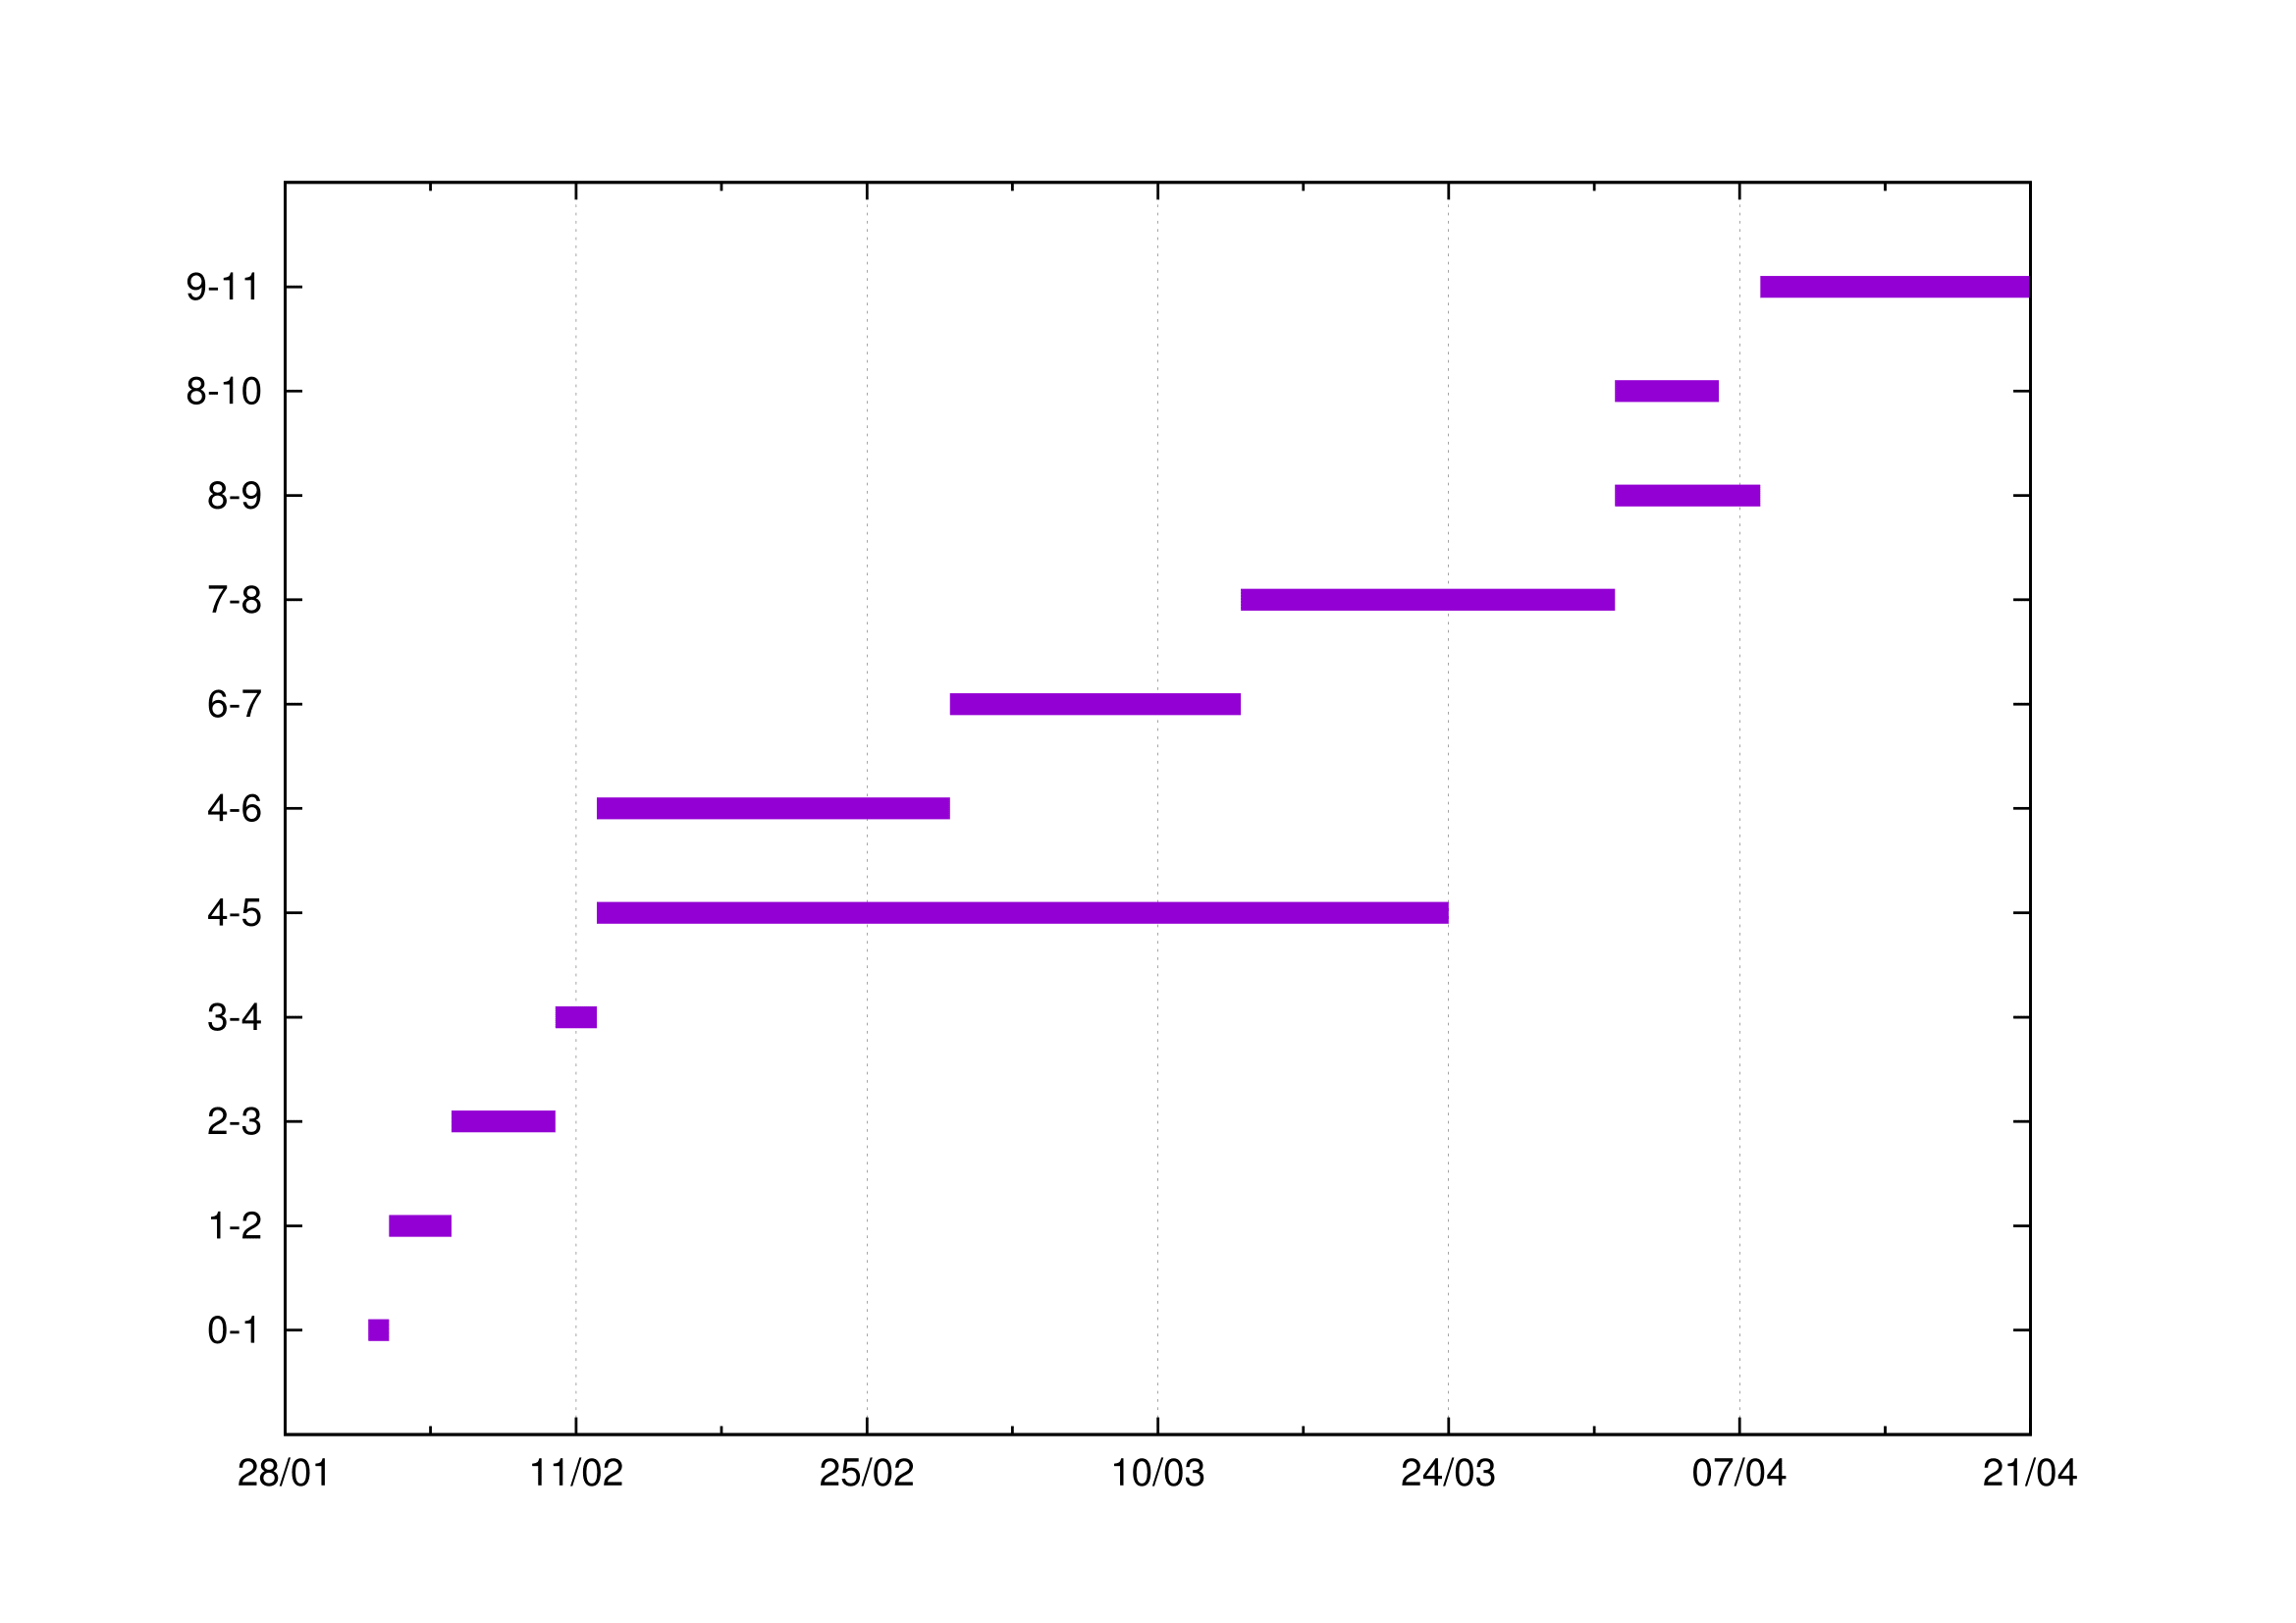
\includegraphics[scale=0.7]{pictures/gantt}
\end{figure}

\begin{table}
\centering
\caption{Таблица занятости исполнителей}
\label{table:time_fond}
\begin{tabular} {| l | l | l | l |} 
\hline
Код работы &   Начало & Окончание & Исполнитель\\
\hline
0-1 & 02.02.16 & 02.02.16 & Программист\\
\hline
1-2 & 03.02.16 & 05.02.16 & Программист\\
\hline
2-3 & 08.02.16 & 10.02.16 & Программист\\
\hline
3-4 & 11.02.16 & 12.02.16 & Программист\\
\hline
4-5 & 15.02.16 & 24.03.16 & Программист\\
\hline
4-6 & 15.02.16 & 29.02.16 & Инженер\\
\hline
6-7 & 01.03.16 & 14.03.16 & Программист\\
\hline
7-8 & 15.03.16 & 01.04.16 & Программист\\
\hline
8-9 & 04.04.16 & 08.04.16 & Инженер\\
\hline
8-10 & 04.04.16 & 06.04.16 & Программист\\
\hline
9-11 & 11.04.16 & 21.04.16 & Инженер\\
\hline
\end{tabular}
\end{table}
